\documentclass[10pt,conference]{IEEEtran}
\IEEEoverridecommandlockouts
% The preceding line is only needed to identify funding in the first footnote. If that is unneeded, please comment it out.
\usepackage{cite}
\usepackage{amsmath,amssymb,amsfonts}
%\usepackage{algorithmic}
\usepackage{graphicx}
\usepackage{textcomp}
\usepackage{xcolor}
\usepackage{tikz}
\usepackage{multirow}
\usetikzlibrary{arrows.meta}
\usepackage{subcaption}
\usepackage{todonotes}
\usepackage{multirow}
\usepackage{xspace}
\usepackage{hyperref}
\usepackage{url}
\usepackage{comment}
\usepackage{listings}

\def\BibTeX{{\rm B\kern-.05em{\sc i\kern-.025em b}\kern-.08em
    T\kern-.1667em\lower.7ex\hbox{E}\kern-.125emX}}
\begin{document}

\newcommand\schim{SchIM\xspace}
\newcommand\schimL{Scheduler In-the-Middle\xspace}
\newcommand\schiml{scheduler in-the-middle\xspace}
\newcommand\axiin[1]{$\texttt{HPM}_{#1}$\xspace}
\newcommand\axiout[1]{$\texttt{HPS}_{#1}$\xspace}
\newcommand\axiconf[1]{$\texttt{LPM}_{#1}$\xspace}

\newcommand{\fig}[1]{Fig.~\ref{#1}}

\newcommand*\circledfig[2]{Fig.~\ref{#1}\tikz[baseline=0pt]{\node[anchor=south west,red,shape=circle,draw,inner sep=1pt] (char) {\scriptsize#2};}}

\newcommand*\circled[1]{\tikz[baseline=0pt]{\node[anchor=south west,red,shape=circle,draw,inner sep=1pt] (char) {\scriptsize#1};}}

\title{
    Work in Progress: Experimenting with Non-blocking Shared Caches on MPSoC platform
%    \thanks{Identify applicable funding agency here. If none, delete this.}
}

\author{
%    \IEEEauthorblockN{1\textsuperscript{st} Given Name Surname}
%    \IEEEauthorblockA{
%        \textit{dept. name of organization (of Aff.)} \\
%        \textit{name of organization (of Aff.)}\\
%        City, Country \\
%        email address or ORCID
%    }
%    \and
%    \IEEEauthorblockN{2\textsuperscript{nd} Given Name Surname}
%    \IEEEauthorblockA{
%        \textit{dept. name of organization (of Aff.)} \\
%        \textit{name of organization (of Aff.)}\\
%        City, Country \\
%        email address or ORCID
%    }
%    \and
%    \IEEEauthorblockN{3\textsuperscript{rd} Given Name Surname}
%    \IEEEauthorblockA{
%        \textit{dept. name of organization (of Aff.)} \\
%        \textit{name of organization (of Aff.)}\\
%        City, Country \\
%        email address or ORCID
%    }
    Authors omitted for review.
}

\maketitle

\begin{abstract}
    In modern real-time multicore systems, understanding and adequately managing shared caches is important to ensure the temporal isolation of critical tasks.
    Recent research has identify and extensively study the sources of unpredictability imputable to shared caches, heavily promoting techniques such as cache partitioning and internal sub-component management.

    In this article, we highlight the existence of an enigmatic source of inter-core interferences. Experiments realised on a development board show that benchmarks (issued from the San-Diego Vision Benchmark Suite) can see their execution time multiplied by 10. The same experiment shows that for extreme cases the core cluster can be stalled indefinitely.
\end{abstract}

\begin{IEEEkeywords}
    Multi-processors Systems, Real-Time Systems, Non-blocking Caches
\end{IEEEkeywords}

\section{Introduction}
    In modern embedded Mutli-core Systems, caches have become an angular piece of hardware bridging the gap between the speed of the connected execution units and the main memory. With the growing demand for high-performance multi-core system on chips, shared caches have evolved to accomodate the many concurrent accesses to main memory and increase the cache hit-rate. These caches are referred to as \emph{non-blocking}.\\

    Unfortunately, while non-blocking shared caches offer great average perfomance, their behaviour is opaque and unpredictable. Dealing with the cache behaviour is of the utmost importance for safety critical hard Real-Time systems where timing constraints must be respected and guaranteed. A great deal of research has been conducted on cache management for Real-Time applications on MPSoCs. The two main sources of unpredictability imputed to the last-level of cache are (1) the inter-core cache line eviction and (2) the opaque management of internaly shared resources.

    The inter-core cache line eviction is a well studied source of unpredictability that arises when the memory accesses of two independent cores lead to the eviction of each others cache line in a destructive way. Such source of unpredictability can be addressed and mitigated by enforcing the \emph{spacial isolation} of the cores. Both software solutions (e.g. via cache coloring \cite{}) and hardware solutions (e.g. via lockdown per master \cite{Giovani_cahe_partitioning_survey}) are available and commonly used.

    Inter-core interferences caused by internal shared resources such as the \emph{Miss-Status-Holding-Registers} (MSHR) or the \emph{write-back} unit  have been recently studied. In \cite{Valsan2017AddressingIC, Heechul_DDOS_attacks_on_shared_cache}, the authors have shown that these shared resources can introduce a consequent amount of interference, mutiply the exeuction time of the tasks running on the victim core by a factor of 346. Such conditions only occur when the attacker creates extrem contention in the write-back unit, resulting in a head-of-the-line-blocking.\\

    In the present article, we show that on the ARM Cortex-A53 \cite{ARM-cortex-A53} a third source of inter-core interferences exists: the target memory response time. In addition, we demonstrate that, in contrary to what has been shown before, read transactions can also caused interferrences. More accurately, we show that if a target memory ackownledges the transaction, but waits to deliver the response, the execution time of tasks running on independent cores can be impacted by a factor of 11. Furthermore, we show that if this single read transaction is acknowledged by the target memory, but the latter never provides a response, the whole core cluster is frozen indefinitely. To the best of our knowledge, this is the first report demonstrating that a core cluster can be subject to interferences caused by a single isolated read transaction.\\

    The present article is organised as follows: TODO

\section{Background}
    \subsection{Non-blocking Caches}
%        Caches in modern MPSoCs are a crucial component that efficiently bridges the gap between the speed of the execution units and the main memory.
%        However, as good as they are at providing high bandwidth, \emph{blocking caches} are ineffective at hiding cache-miss penaty because they stall the execution units until the data is received from the main memory.
%        In order to hide this penalty and improve the cache performance, \cite{Kroft} proposed the first \emph{Miss-Handling-Architecture} (MHA).
%        This type of cache referred to as \emph{Non-blocking} relies on the introduction of a set of new registers called \emph{Miss Status Holding Register} (MSHR), which are in charge of tracking the status of cache line misses.
%        Each MSHR stores important information regarding the cache-miss such as the target address and the location of the cache line to refill.
%        For each level of cache in a system, the amount of MSHRs denotes the number of outstanding (i.e. simultaneous) transactions it can handle.
%        %This amount is known as the \emph{Memory-Level-Parallelism} (MLP).
%
%        At run time, a non-blocking cache behaves as follows. When a cache-miss occurs, the metadata of the cache-miss is stored in one of the available MSHRs. In case the same cache-miss already occurred and one MSHR already holds the metadata, the two requests are merged.
%        It is only once the cache line refill request has been served and placed in the proper cache line that the MSHR is made available to store new cache-misses requests.
%        Provided that all the MSHRs are used at a given instant, the system stops until one of them becomes available.

        Caches in modern MPSoCs are a crucial component that efficiently bridges the gap between the speed of the execution units and the main memory.
        However, as good as they are at providing high bandwidth, \emph{blocking caches} are ineffective at hiding cache-miss penalty because they stall the execution units until the data is received from the main memory.
        In order to hide this penalty and improve the cache performance, \cite{Kroft} proposed the first \emph{Miss-Handling-Architecture} (MHA).
        This type of cache referred to as \emph{Non-blocking} relies on the introduction of a set of new registers called \emph{Miss Status Holding Register} (MSHR), which are in charge of tracking the status of cache line misses.
        Each MSHR stores important information regarding the cache-miss such as the target address and the location of the cache line to refill.
        For each level of cache in a system, the amount of MSHRs denotes the number of outstanding (i.e. simultaneous) transactions it can handle.
        %This amount is known as the \emph{Memory-Level-Parallelism} (MLP).

        At run time, a non-blocking cache behaves as follows. When a cache-miss occurs, the metadata of the cache-miss is stored in one of the available MSHRs. In case the same cache-miss already happened and one MSHR already holds the metadata, the two requests are merged.
        It is only once the cache line refill request has been served and placed in the proper cache line that the MSHR is made available to store new cache-misses requests.
        If all the MSHRs are used, the system stops until one of them becomes available.

    \subsection{Programmable Logic In the Middle (PLIM)}
%        The \emph{Programmable Logic In the Middle} (PLIM) is a new paradigm introduced by \cite{PLIM20} that takes advantage of the newly available platforms associating a traditional \emph{Processing System} (PS side) with a tightly integrated Programmable Logic (PL side).
%        In a system using PLIM, the PL side is leveraged such that the latter is located in between the core cluster and the main memory in the data path.
%        In other words, a PLIM module is a piece of custom logic located on the PL side that is capable of manipulating the transactions coming from the core cluster before they reach the main memory.
%        For instance, \cite{PLIM20} tackled important constraints imposed by the cache coloring technique by using a PLIM module (called \emph{bleacher}) by applying a configurable transformation on each incoming transaction address.
%        The use of a PLIM module broadens considerably the control over memory operations as it becomes possible to manipulate the memory traffic generated by the core cluster at the granularity of individual transactions.

        The \emph{Programmable Logic In the Middle} (PLIM) is a new paradigm introduced by \cite{PLIM20} that takes advantage of the newly available platforms associating a traditional \emph{Processing System} (PS side) with a tightly integrated Programmable Logic (PL side).
        In a PLIM system, the PL side is located in the middle of the data path, between the core cluster and the main memory.
        In other words, a PLIM module is a piece of custom logic located on the PL side that is capable of manipulating the transactions coming from the core cluster before they reach the main memory.
        For instance, \cite{PLIM20} tackles significant constraints imposed by the cache coloring technique by using a PLIM module (called \emph{bleacher}) by applying a configurable transformation on each incoming transaction address.
        Using a PLIM module broadens the control over memory operations considerably as it becomes possible to manipulate the memory traffic generated by the core cluster at the granularity of individual transactions.

\section{Related work}
    An important amount of research has focused on addressing the challenges of isolating the cores sharing the same cache and thus, preventing unpredictable behaviour such as increased in execution time.
    Most of this research \cite{Mancuso2013RealtimeCM, 6755286} has aimed at \emph{spacially isolating} the cores (i.e. avoiding inter-core cache line eviction by constraining each core data and instructions in a specific region of the shared cache). Hardware based solutions such as \emph{lockdown per way} \cite{Giovani_cahe_partitioning_survey} are efficient, but not integrated in every platforms.
    On the other hand, software based solutions such as cache coloring \cite{Mancuso2013RealtimeCM} can be deployed in most platforms, but comes at the cost of increased memory space requirements.

    However, recent research \cite{Valsan2017AddressingIC, Heechul_DDOS_attacks_on_shared_cache} have highlighted that, while cache partitioning is successful in most cases, in some situations, contention on shared internal units such as the MSHRs or the write-back unit can also introduce substential inter-core interferences.
    In \cite{Valsan2017AddressingIC}, the authors evaluate the impact of inter-core interference originated by the MSHRs on multiple platforms and propose a solution to eliminate this contention. The solution is based on a combination of a small hardware module and an OS-level controller.
    Their experiments show that, if let unmanaged, the execution time of independent cores is multiplied by 10.6 and 21.3 under read and write workloads, respectively.
    By the mean of simulation, they prove that their approach is successful at providing the best overall throughput for each core while suppressing the inter-core interference caused by the MSHRs.
    % Running applicative benchmarks, increas in execution time of a factor of 6.4 have been observed.
    \cite{Heechul_DDOS_attacks_on_shared_cache} investigates the contention in caches caused by shared internal units in the case of \emph{Denial-of-service} (DOS) attacks and propose an OS-level solution enabling finer management of the system bandwidth.
    In contrast to \cite{Valsan2017AddressingIC}, the internal unit studied and exploited is the write-back unit.
    They report that, by exploiting this unit efficiently, one can increase the execution time of a victim task by a factor of 346.

\section{System Model}
    \label{sec:system_model}

%    As a model, we consider a PS-PL system where the processing system must feature at least two cores and a shared non-blocking LLC.
%    The PL side is programmed with a PLIM module called the AXI-Resistor as depicted in Figure \ref{fig:system_schematic}, which will act as a slow cacheable memory target (more details in Section \ref{subsec:axi-resistor}).
%    The platform resources are shared between two actors: a \emph{victim} and an \emph{attacker}.
%    In the present scenario, the victim executes a set of tasks addressing directly the main memory (i.e. the path highlighted in red in Figure \ref{fig:system_schematic}), whereas the attacker mainly targets the AXI-Resistor with read transactions.
%    Figure \ref{fig:system_schematic} offers a schematic representation of the platform and how it is used for the experiment.

%    As a model, we consider a PS-PL system where the processing system must feature at least two cores and a shared non-blocking LLC.

%    As displayed in Figure \ref{fig:system_schematic}, the system model is a PS-PL system where the processing system is composed of four cores and a shared non-blocking LLC.
%    The PL side is programmed with a PLIM module, called the AXI-Resistor, which acts as a slow cacheable memory target (more details in Section \ref{subsec:axi-resistor}).
%    The platform resources are shared between two actors: a \emph{victim} and an \emph{attacker}.
%    In our scenario, the victim executes a set of tasks addressing the main memory (i.e., the path highlighted in red in Figure \ref{fig:system_schematic}), whereas the attacker mainly targets the AXI-Resistor with read transactions.
%%    Figure \ref{fig:system_schematic} offers a schematic representation of the platform and its use for the experiment.

    The system model assumed in this paper is composed of two isolated actors: a \emph{victim} and an \emph{attacker}.
    On one hand, the victim is defined as a set of trusted applications having to meet specific deadlines.
    On the other hand, the attacker is a lightweight application in charge of disturbing the victim.
    The attack consists in a continuous flow of single sequential read transactions emitted towards a slow memory, the AXI-Resistor.

    This section is divided into three parts, each giving further details on the system model components.
    First, in Section \ref{subsec:processing_system_organization} details regarding the isolation of the actors are given.
    Secondly, a complete description of the attacker's design is provided in Section \ref{subsec:attacker_design}.
    Finally, Section \ref{subsec:axi-resistor} explains the AXI-Resistor architecture and mechanism.

    \subsection{Processing System Organization}
        \label{subsec:processing_system_organization}
        As displayed in Figure \ref{fig:system_schematic}, the actors are located on the same core cluster but are allocated non-overlapping sets of resources.
        In other words, they run on different cores and have private LLC partitions.
        This measure enforces the independence of the two actors and ensures that the observed interference cannot be imputed to either a common software stack or inter-core cache line evictions.
        Moreover, the private LLC partition of the attacker is subdivided into two.
        The first half allows the attacker to access the main memory, where its code is located (via the red path in Figure \ref{fig:system_schematic}), whereas the second half is dedicated to the data read through the AXI-Resistor (via the orange route in Figure \ref{fig:system_schematic}).

        Assuming the attacker accesses to the main memory introduce little to no inter-core interference, the two actors can be deemed as properly isolated.

%    This Section presents the details of the different components and actors of the experiment.
%    Further details regarding the organization of the PS side are given in Section \ref{subsec:processing_system_organization}.
%    In section \ref{subsec:attacker_reading_memory_bomb}, a description of the attacker is given.
%    Finally, the implementation and the characteristics of the AXI-Resistor are discussed in Section \ref{subsec:axi-resistor}.

%    \subsection{Processing System Organization}
%        \label{subsec:processing_system_organization}
%%        As previously mentioned, the PS side and especially the core cluster is shared by both the victim and the attacker.
%%        We assume a partitioned system where each actor is assigned a given set of cores and a private partition of the LLC.
%%        Consequently, each actor is independent, ensuring that the observed delays cannot be imputed to either a common software stack or inter-core cache line evictions.
%%
%%        On one hand, we define our victim actor as a set of trusted applications and controllers having to meet certain deadlines.
%%        On the other hand, we define our attacker actor as a lightweight application in charge of emitting sequential read transactions toward the desired target.
%%        As shown in Figure \ref{fig:system_schematic}, the attacker splits its private partition of the LLC in two.
%%        The first one half allows the attacker to access the main memory, where its code is located (via the path highlighted in red in Figure \ref{fig:system_schematic}) and the second half is dedicated to the data read through the AXI-Resistor (the orange path in Figure \ref{fig:system_schematic}).
%%        Isolating the two address spaces is important as it enables a direct control over the amount of transactions targeting the AXI-Resistor.
%%
%%        Globally, the actors are perfectly isolated.
%%        The only exception being that the attacker also access the main memory to fetch its code.
%%        Nonetheless, this should introduce little or no inter-core interference.
%
%        To enforce the independence of the victim and the attacker actors, we partition the the PS side by assigning them a specific set of cores and a private cache partition.
%        This measure ensures that the observed delays cannot be imputed to either a common software stack or inter-core cache line evictions.
%
%        On one hand, we define our victim actor as a set of trusted applications and controllers having to meet specific deadlines.
%        On the other hand, we define our attacker actor as a lightweight application in charge of emitting sequential read transactions toward the desired target.
%        As shown in Figure \ref{fig:system_schematic}, the attacker splits its private partition of the LLC in two.
%        The first half allows the attacker to access the main memory, where its code is located (via the path highlighted in red in Figure \ref{fig:system_schematic}). The second half is dedicated to the data read through the AXI-Resistor (the orange path in Figure \ref{fig:system_schematic}).
%        Isolating the two address spaces enables a precise control over the number of transactions targeting the AXI-Resistor.
%
%%        Globally, the actors are perfectly isolated.
%%        The only exception is that the attacker also accesses the main memory to fetch its code.
%%        Nonetheless, this should introduce little or no inter-core interference.
%
%        Assuming the attacker's accesses to the main memory introduce little to no inter-core interference, the two actors can be deemed as properly isolated.

    \subsection{Attacker's Design}
        \label{subsec:attacker_design}
%        Even with the aforementioned precautions, the design of the attacker (i.e. the read memory bomb) must be thought carefully.
%        In fact, if not under control a read memory bomb will steadily fetch data, creating many cache-misses.
%        Following the non-blocking cache mechanism, these cache-misses will be inserted in one of the available MSHRs until all of them are used.
%        In this situation the non-blocking cache controller will stop the whole machinery, leading to the phenomenon reported by \cite{Heechul_DDOS_attacks_on_shared_cache}.
%        %
%        This effect can only be avoided by throttling down the attacker core.
%        We enforce this by following each read request by a \emph{Data Synchronization Barrier} (\texttt{DSB}).
%        This ensures that at each instant, there will not be more than one transaction targeting the AXI-Resistor and, by extension, it guarantees at most one MSHR is occupied by the attacker actor.

        Even with the precautions mentioned in Section \ref{subsec:processing_system_organization} (i.e., actors isolation), the design of the attacker must be thought carefully to highlight the CPU-brainfreeze. % (i.e., the read memory bomb)
        As, if not under control, a read memory bomb will steadily fetch data, creating many cache-misses.
        Following the non-blocking cache mechanism, these cache-misses will be inserted in one of the available MSHRs until all of them are used.
        In this situation, the non-blocking cache controller will stop the whole machinery, leading to the phenomenon reported by \cite{Valsan2017AddressingIC}.

        This effect can only be avoided by throttling down the attacker's core.
        We enforce this by following each read request by a \emph{Data Synchronization Barrier} (\texttt{DSB}).
        This instruction ensures that at each instant, there will not be more than one transaction targeting the AXI-Resistor and, by extension, it guarantees at most one MSHR is occupied by the attacker.

    \subsection{AXI-Resistor IP}
        \label{subsec:axi-resistor}
%        In our system model, the AXI-resistor IP is a PLIM module \cite{PLIM20} used to act as a slow cacheable memory target.
%        Typically, the IP accepts every read transaction coming from the core cluster via the HPM port, buffers them and only release them one by one in direction of the DRAM controller.
%        Releases are spaced by a minimal inter-arrival time (MIT) expressed in clock cycles (CC).
%        This data path is highlighted in orange in Figure \ref{fig:system_schematic}.
%        Because each transaction is intercepted by the AXI-Resistor before arriving to the DRAM controller, the latter is unaware of the transaction and no internal mechanism is activated, suppressing potential interference induced by the DRAM controller.
%
%        The AXI-Resistor is composed of three ports: one slave port accepting transactions from the core cluster, one configuration port (blue route in Figure \ref{fig:system_schematic}) and one master port relaying the transactions out of the IP.
%        Arriving transactions are buffered within the AXI-Resistor thanks to a queue (see \emph{Addresss Phase Lane} on the right of Figure \ref{fig:system_schematic}).
%        The transaction stored at the head of the queue is released according a timer.
%        The period of this timer is reprogrammable at run-time thanks to the configuration port.
%        Once a read request has been served by the DRAM controller, the read data is sent back to the core cluster through the AXI-Resistor.
%        This phase is not buffered by the IP as shown in Figure \ref{fig:system_schematic} (see \emph{Response Phase Lane}).

%        In our system model, the AXI-resistor IP is a PLIM module \cite{PLIM20} used to act as a slow cacheable memory target.
%        Typically, the IP accepts every read transaction coming from the core cluster via the HPM port, buffers them, and only releases them one by one toward the DRAM controller.
%        Transaction releases are seperated by a minimal inter-arrival time (MIT) expressed in clock cycles (CC).
%        This data path is highlighted in orange in Figure \ref{fig:system_schematic}.
%        Because the AXI-Resistor intercepts each transaction before they reach the DRAM controller, the latter is unaware of the transactions.
%        Consequently, no internal mechanism is activated, suppressing potential interference induced by the DRAM controller.
%
%        The AXI-Resistor is composed of three ports: one slave port accepting transactions from the core cluster, one configuration port (blue route in Figure \ref{fig:system_schematic}), and one master port relaying the transactions out of the IP.
%        Arriving transactions are buffered within the AXI-Resistor thanks to a queue (see \emph{Addresss Phase Lane} on the right of Figure \ref{fig:system_schematic}).
%        The transaction stored at the head of the queue is released according to a timer.
%        The period of this timer is reprogrammable at run-time thanks to the configuration port.
%        Once the DRAM controller has served a read request, the data read is sent back to the core cluster through the AXI-Resistor.
%        This phase is not buffered by the IP as shown in Figure \ref{fig:system_schematic} (see \emph{Response Phase Lane}).

    In our system model, the AXI-Resistor is a PLIM module \cite{PLIM20} located on the secondary route to the main memory (see the orange route in Figure \ref{fig:system_schematic}) and used to act as a slow cacheable target memory.
    In addition, the AXI-Resistor also prevents any potential interference introduced by the DRAM controller as the former intercepts every transaction before they reach the latter.

    The mechanism enabling the characteristics mentioned just above is the following.
    Upon the reception of a read transaction coming from the core cluster via the HPM port, the IP inserts this transaction within a queue where it waits to be relayed out of the AXI-Resistor.
    The decision to relay the transaction stored at the head of the queue to the DRAM controller is done according to a timer.
    The latter is located within the AXI-Resistor (see \emph{Configuration} in Figure \ref{fig:system_schematic}) and, from the DRAM controller perspective, enforces a minimal inter-arrival time (MIT) between two consecutive transactions.
    The MIT is expressed in clock cycles (CC) and is dynamically reprogrammable thanks to a configuration port accessible by all cores with uncached transactions (see the cyan route in Figure \ref{fig:system_schematic}).
%        In contrast to the transactions heading to the DRAM controller via the AXI-Resistor, transactions served by the DRAM controller and returning to the core cluster traverse the AXI-Resistor without being buffered (see \emph{Response Phase Lane} in Figure \ref{fig:system_schematic}).

\section{Results}
    \label{sec:results}
    \begin{figure*}
        \centering
        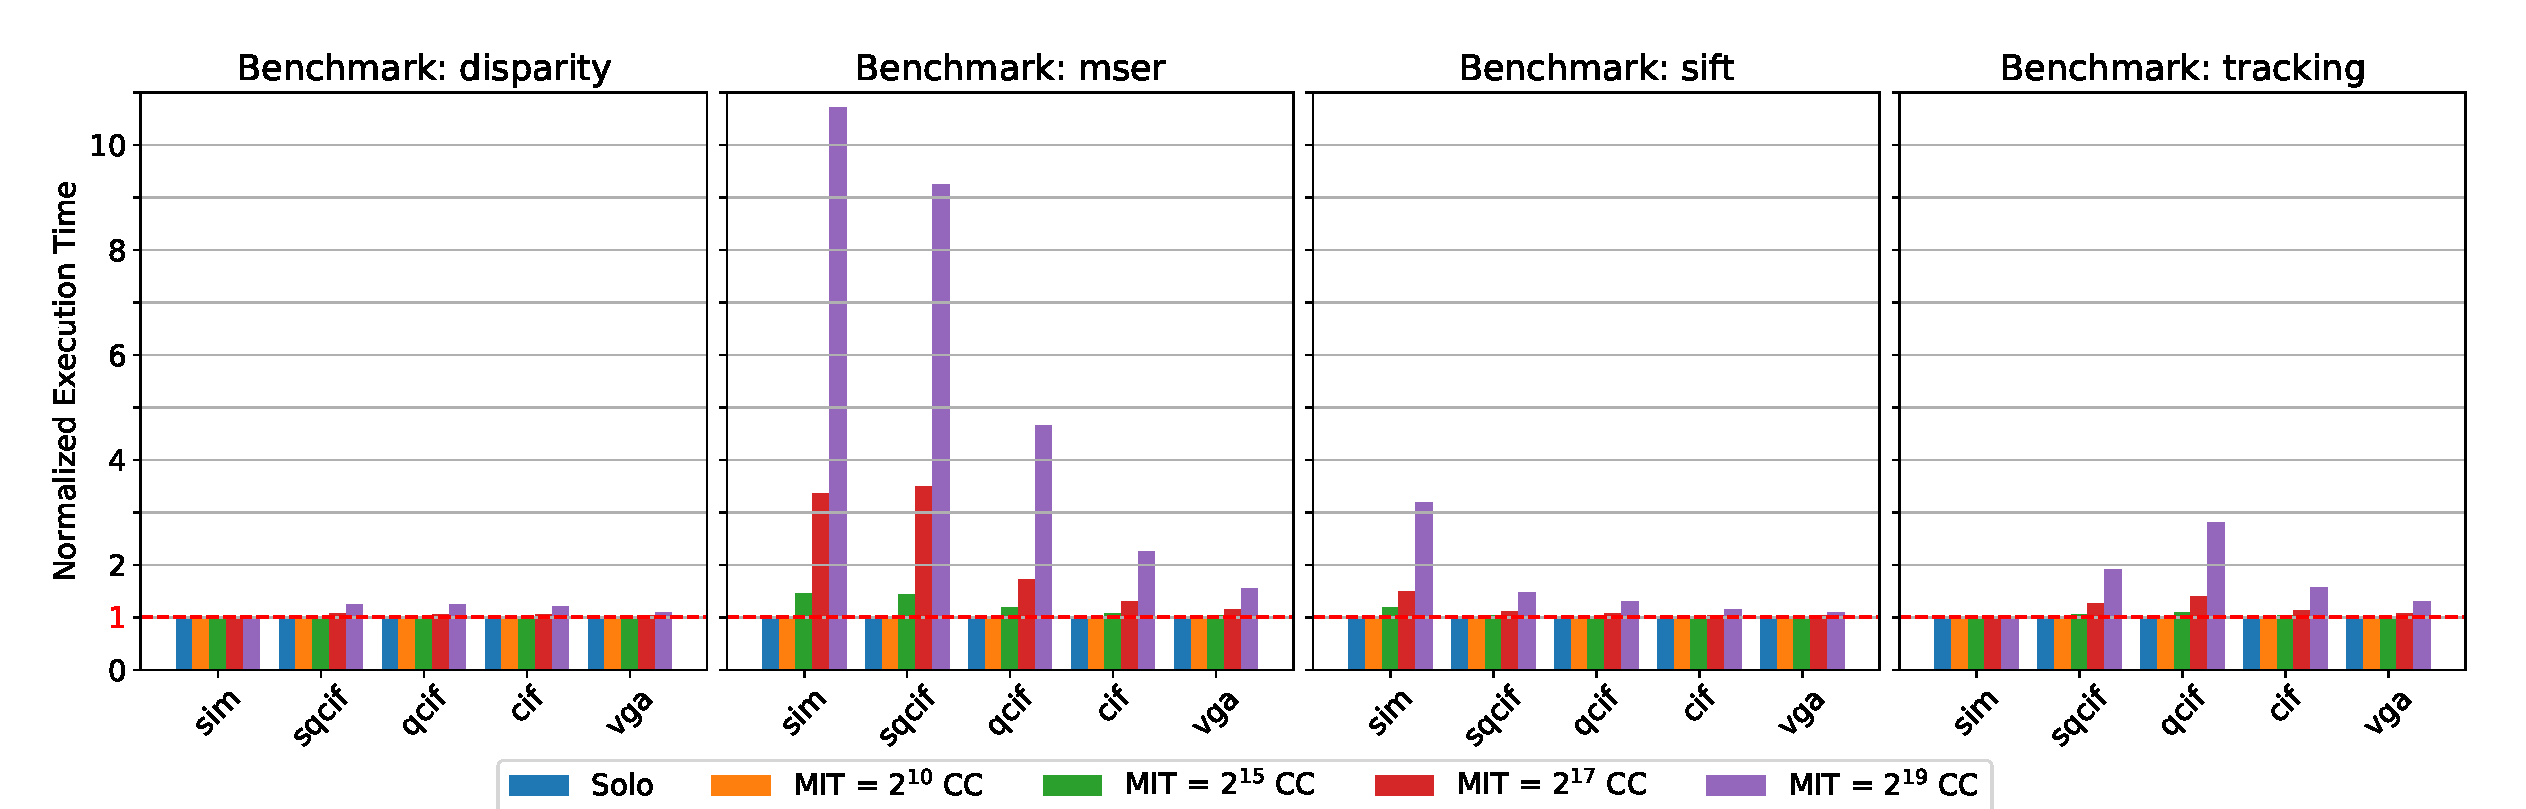
\includegraphics[scale=0.425]{images/cpu-brainfreeze-interference.pdf}
        \caption{}
        \label{fig:cpu-brainfreeze-interference-results}
    \end{figure*}

    \begin{table}
        \centering
        \caption{}
        \label{tab:sd-vbs-input-sizes}
        \begin{tabular}{|l||c|c|c|c|c|}
            \hline
            Input size name  & \emph{sim} & \emph{sqcif} & \emph{qcif} & \emph{cif} & \emph{vga} \\
            \hline
            Size in Kilobytes &  $11.7$ &    $36.9$ &   $81.4$ & $304.2$ & $846.8$ \\
            \hline
        \end{tabular}
    \end{table}

    Using the scenario and setup presented in section \ref{sec:evaluation_setup}, we aim at observing the interference caused bu the lightweight read attcker on the victim inmate. To this end, we ran few applicative benchmarks issued from the San-Diego Vision Benchmark Suite \cite{SD-VBS} for all the available input sizes. The benchmarks were also run ffor different configuration of the AXI-Resistor. The latter was configured with MITs of $2^{10}$, $2^{15}$, $2^{17}$ and $2^{19}$. As a baseline, the benchmarks have also been run alone (i.e. without an attacker). This baseline is referred to as "Solo" in Figure \ref{fig:cpu-brainfreeze-interference-results}.

    Figure \ref{fig:cpu-brainfreeze-interference-results} offers a relevant subset\footnote{The complete set of results is available at: URL ommited for review} of results obtained from the experiment. All the results for a given benchmark (localization, mser, sift and tracking) and its size input (see Table \ref{tab:sd-vbs-input-sizes}) have been normalized with respect to the equivalent combination running alone (i.e. Solo, the leftmost blue bar in each bar cluster).

    As display in Figure \ref{fig:cpu-brainfreeze-interference-results}, the victim inmate, while running the localization benchmark, suffers from little to no interference from the attacker. The only noticeable increase in execution time is for a \emph{vga} input size and a MIT of $2^{19}$, where the victim suffers from a $150\%$ increase of computation time.
    On the other hand, when running mser, a well known memory bound benchmark, noticeable increases in execution time are observed, with a factor of 10 observed for the \emph{sim} input size.
    For both sift and tracking spikes in execution time are observed. Eventhough, there is no clear pattern with respect to the input sizes, increase in execution time happen for MITs of $2^{17}$ and $2^{19}$.\\

    Interrestingly, configuring the AXI-Resistor in such a way that it would accept the read trasaction, but never answer systematically, leads to the whole system being suspended undefinitely. This can effectively be considered as a Denial-of-Service attack.

\section{Discussion}
    Non-blocking caches are advertised as cache units capable of hiding the cache hit-miss penalty and managing multiple simultaneous memory accessses created by the cores in a seamless fashion (i.e. without stalling the whole core cluster at each miss) unless all the MSHRs are used or the write-back unit buffer is full. Nothing in the non-blocking cache architecture suggests that a single outstanding read transaction could introduce inter-core interferences. However, our experiment tends to show the opposite.

    While the exact source of the observed inter-core interferences is unclear to the authors, all the precautions taken during the experiment (i.e. isolation of the inmates and partition of the cache) and the result tend to suggest that the source originates from the LLC controller itself.

    The authors acknowledge that the described phenomenon is unlikely to occur in a normal situation (i.e. all the inmates target the main memory), and if it does, the consequences should be negligeable.
    Nonetheless, this experiment has the merit of pinpointing a malfunction in the LLC controller of the ARM Cortex-A53.
    It is a reminder of the gap between the theoretical models, the hardware behaviour expectations and the real behaviour of the hardware.

%    The experiment also sheds light on the importance of selecting trustable third party IPs and designing correctly IPs if they aim to be cacheable target memories.
%    Any bus slaves must be designed carefully in order to provide fast answers. This is specially the case for PLIM modules which aim at being cacheable targets.
%    Finally, software stacks provided with SoCs featuring a tightly integrated programmable logic must ensure that the latter can only be reprogrammed by a trusted actor as simply holding a single cached read transaction can indefinitely stall the whole core cluster.

\section{Conclusion}
    \begin{itemize}
        \item Such system, under strict conditions cannot quarantee QoS nor Mixed-criticality levels.
        \item In contrast to what has been previously reported, read intensive applications can also become a threat for the system predictability.
    \end{itemize}
    \subsection{Future works}
        \begin{itemize}
            \item Study if the same impact can be found with the attacker targeting a scratch pad memory which frequency could be modify.
            \item Investigate whether this phenomenom can also be observed in other, more recent, ARM core families.
        \end{itemize}


\bibliographystyle{IEEEtranS}
\bibliography{references}

\end{document}
